%
% einleitung.tex -- Beispiel-File für die Einleitung
%
% (c) 2020 Prof Dr Andreas Müller, Hochschule Rapperswil
%
% !TEX root = ../../buch.tex
% !TEX encoding = UTF-8
%
\section{Theorie\label{reynolds:section:teil0}}
\kopfrechts{Theorie}
\subsection{Die Navier-Stokes-Gleichungen}

Im folgenden Abschnitt wird kurz erläutert, wie man von den berühmten Navier-Stokes-Gleichung
durch mathematische Umformungen auf die zeitgemittelten RANS-Gleichungen kommt.

Ziel dieser Umformungen ist es, die Möglichkeit zu schaffen, mittels zusätzlicher Felder
die mittleren Effekte von Eddies zwischen zwei Zeitschritten so zu beschreiben, dass sich die
Effekte in die Navier-Stokes-Gleichungen einfügen lassen.



Die Navier-Stokes-Gleichungen für ein viskoses, inkompressibles, newtonisches Fluid lauten

\begin{align}
    \label{reynolds:eqs:mass}
    \frac{\partial u_i}{\partial x_i} &= 0 \\
    \label{reynolds:eqs:impulse}
    \frac{\partial u_i}{\partial t} + u_j \frac{\partial u_i}{\partial x_j} &=
        f_i - \frac{1}{\rho} \frac{\partial p}{\partial x_i} + 
        \nu \frac{\partial^2 u_i}{\partial x_j \partial x_j}, \text{für $i = 1,2,3$}
\end{align}

Die Gleichungen machen Gebrauch von der ``Euler-Notation'': Über Indizes, welche in einem Term doppelt
erscheinen, wird summiert, so entspricht z.B. in Gleichung \ref{reynolds:eqs:impulse}

\begin{equation}
u_j \frac{\partial u_i}{\partial x_j} = \sum_{j=1}^{3} u_j \frac{\partial u_i}{\partial x_j}
\end{equation}

Die Terme lassen sich wie folgt beschreiben:

\begin{enumerate}
    \item $\frac{\partial u_i}{\partial x_i} = \operatorname{div}(\mathbf{u})$: ``Massengenerierung''.
    Aufgrund des Massenerhalts $ = 0$.
    \item $\frac{\partial u_i}{\partial t}$: Die zeitliche Änderung der Flussgeschwindigkeit (also die 
        Impulsänderung) and einem fixen, örtlichen Punkt.
    \item $u_j \frac{\partial u_i}{\partial x_j}$: Die Konvektion, also die Impulsänderung durch ``Abfliessen''
        von bewegten Teilchen.
    \item $f_i$: Andere, allgemeine ``innere'' Kräfte, typischerweise die Gravitation.
    \item $\frac{1}{\rho} \frac{\partial p}{\partial x_i}$: Das Druckgefälle.
    \item $\nu \frac{\partial^2 u_i}{\partial x_j \partial x_j}$: Die Diffusion, also Änderung des Impulses
        aufgrund mikroskopischer Kollisionen und anderer Wechselwirkungen von Teilchen bzw.
        makroskopischer Reibung.
\end{enumerate}

\subsection{Die Reynolds-Zerlegung}

Für eine gegebene zeitliche Schrittgrösse $\Delta t$ wird die Reynolds-Zerlegung von $u_i$ zur Zeit $t = t_0$
wie folgt definiert:

\newcommand{\ravg}[1]{\left\langle #1 \right\rangle}
\newcommand{\rdecomp}[1]{\ravg{#1} + #1'}

\begin{equation}
    \label{reynolds:eqs:reynolds-decomp}
    u_i = \rdecomp{u_i}
\end{equation}

wobei der Operator $\ravg{\cdot}$ wie folgt definiert ist

\begin{equation}
    \ravg{g} = \frac{1}{\Delta t}\int_{t=t_0}^{t_0 + \Delta t} g \mathrm{\,d}t
\end{equation}

für eine beliebige Funktion $g$.

$u_i(t)$ wird also in den mittleren Teil $\langle u_i \rangle$, welcher über den Zeitraum
$\Delta t$ konstant bleibt, und den transienten teil $u_i'(t) = u_i(t) - \langle u_i \rangle$
zerlegt.

Aus der Definition des Operators $\langle \cdot \rangle$ folgen die Eigenschaften:

\begin{align}
    \ravg{\ravg{a}} &= \ravg{a} \\
    \ravg{a + b} &= \ravg{a} + \ravg{b} \\
    \ravg{a \ravg{b}} &= \ravg{a} \ravg{b} \\
    \ravg{\frac{\partial a}{\partial \cdot}} &= \frac{\partial \ravg{a}}{\partial \cdot}
\end{align}

und daher

\begin{equation}
    \label{reynolds:eqs:trans-cancel}
    \ravg{u_i'} = \ravg{u_i - \ravg{u_i}} = \ravg{u_i} - \ravg{u_i} = 0
\end{equation}

\subsection{Turbulenz}

Turbulenz kann auf sehr kleinen zeitlichen und räumlichen Skalen auftreten.
Insbesondere können diese viel kleiner als $\Delta t$ sein. Um die Turbulenz in dieser
Grössenordnung abbilden zu können, wird eine sehr kleine zeitliche und räumliche Diskretisierung
benötigt. Dies führt zu grossem Rechenaufwand. Meistens interessieren die Vorgänge unter
einer gewissen Grössenordnung jedoch nicht. Versucht man aber, einfach den Zeitschritt
(und die Gitterweite) zu erhöhen, ohne die zu lösenden Navier-Stokes-Gleichungen
anzupassen, kann dies zu numerischen Instabilitäten führen.

\subsection{Reynolds-Averaging}
Eine Art, die Gleichungen anzupassen ist ``Reynolds-Averaging''. Mit Reynolds-Averaging verfolgt
man das Ziel, sich auf Phänomene zu fokussieren, die in etwa eine Zeitspanne $\Delta t$ überdauern.
Zeitlich schnellere Phänomene werden über eine Zeit von $\Delta t$ gemittelt.

Im ersten Schritt werden die Unbekannten Geschwindigkeit, $u_\cdot$, und Druck,, $p$ in den Navier-Stokes-Gleichungen
\ref{reynolds:eqs:impulse} durch ihre Reynolds-Zerlegungen - $\rdecomp{u_\cdot}$ und analog für $p$ - ersetzt und die Gleichung
mit $\rho$ multipliziert. Wir erhalten dann

\begin{equation}
    \label{reynolds:eqs:der1}
    \rho \left( \frac{\partial \left( \rdecomp{u_i} \right)}{\partial t} + \rdecomp{u_j} \frac{\partial \left( \rdecomp{u_i} \right)}{\partial x_j} \right) =
        - \frac{\partial \left( \rdecomp{p} \right)}{\partial x_i} + 
        \mu \frac{\partial^2 \left( \rdecomp{u_i} \right)}{\partial x_j \partial x_j}
\end{equation}

mit $\mu = \rho \nu$ und, oBdA, $f_i \equiv 0$.

Mit Hilfe der Produktregel lässt sich der Term $\left( \rdecomp{u_j} \right) \frac{\partial \left( \rdecomp{u_i} \right)}{\partial x_j}$
wie folgt umformen

\begin{equation}
    \left( \rdecomp{u_j} \right) \frac{\partial \left( \rdecomp{u_i} \right)}{\partial x_j} =
        \frac{\partial \left[ \left( \rdecomp{u_j} \right) \left( \rdecomp{u_i} \right) \right]}{\partial x_j}
        - \frac{\partial \left( \rdecomp{u_j} \right)}{\partial x_j} \left( \rdecomp{u_i} \right)
\end{equation}

Aus dem Massenerhalt (Gleichung \ref{reynolds:eqs:mass}) folgt

\begin{equation}
    \frac{\partial \left( \rdecomp{u_j} \right)}{\partial x_j} = 0
\end{equation}

und somit

\begin{equation}
    \label{reynolds:eqs:der2}
    \left( \rdecomp{u_j} \right) \frac{\partial \left( \rdecomp{u_i} \right)}{\partial x_j} =
        \frac{\partial \left[ \left( \rdecomp{u_j} \right) \left( \rdecomp{u_i} \right) \right]}{\partial x_j}
\end{equation}

Setzen wir Gleichung \ref{reynolds:eqs:der2} in Gleichung \ref{reynolds:eqs:der2} ein erhalten wir

\begin{align}
    \rho \left(
            \frac{\partial \left( \rdecomp{u_i} \right)}{\partial t} +
            \frac{\partial \left[ \left( \rdecomp{u_j} \right) \left( \rdecomp{u_i} \right) \right]}{\partial x_j}
        \right) = \\
    \rho \left(
            \frac{\partial \left( \rdecomp{u_i} \right)}{\partial t} +
            \frac{\partial \left[ \ravg{u_i} \ravg{u_j}  + \ravg{u_j} u_i' + u_j' \ravg{u_i} + u_j' u_i'\right]}{\partial x_j}
        \right) = \\
    - \frac{\partial \left( \rdecomp{p} \right)}{\partial x_i} + 
    \mu \frac{\partial^2 \left( \rdecomp{u_i} \right)}{\partial x_j \partial x_j}
\end{align}

Als nächstes wird auf beide Seiten der Gleichung der Operator $\ravg{\cdot}$ angewendet.
Aufgrund von Gleichung \ref{reynolds:eqs:trans-cancel} fallen die transienten Terme somit
weg und es bleibt:

\begin{align}
    \frac{\partial \ravg{u_i}}{\partial x_i} &= 0 \\
    \rho \left(
            \frac{\partial \ravg{u_i}}{\partial t} +
            \frac{\partial \left( \ravg{u_i} \ravg{u_j} + \ravg{u_i' u_j'}\right)}{\partial x_j}
        \right) &=
        - \frac{\partial \ravg{p}}{\partial x_i} + 
        \mu \frac{\partial^2 \ravg{u_i}}{\partial x_j \partial x_j}
\end{align}

Der Term $\rho \frac{\partial \ravg{u_i' u_j'}}{\partial x_j}$ wird auf die andere Seiten
des Gleichheitszeichens in den Term $\frac{\partial^2}{\partial x_j \partial x_j}$ gezogen:

\begin{equation}
    \rho \left(
            \frac{\partial \ravg{u_i}}{\partial t} +
            \frac{\partial \left( \ravg{u_i} \ravg{u_j}\right)}{\partial x_j}
        \right) =
        - \frac{\partial \ravg{p}}{\partial x_i} + 
            \frac{\partial}{\partial x_j} \left(
            \mu \frac{\partial \ravg{u_i}}{\partial x_j} - \rho \ravg{u_i' u_j'}
        \right)
\end{equation}

Mit der Vereinfachung (Kettenregel \& Masserhaltung)

\begin{equation}
    \frac{\partial \left( \ravg{u_i} \ravg{u_j}\right)}{\partial x_j} = \\
        \frac{\partial \ravg{u_i}}{\partial x_j} \ravg{u_j} +
        \ravg{u_i} \frac{\partial \ravg{u_j}}{\partial x_j} = \\
        \frac{\partial \ravg{u_i}}{\partial x_j} \ravg{u_j}
\end{equation}

erhalten wir am Ende

\begin{align}
    \label{reynolds:eqs:rans1}
    \frac{\partial \ravg{u_i}}{\partial x_i} &= 0 \\
    \label{reynolds:eqs:rans2}
    \rho \left(
            \frac{\partial \ravg{u_i}}{\partial t} +
            \frac{\partial \ravg{u_i}}{\partial x_j} \ravg{u_j}
        \right) &=
        - \frac{\partial \ravg{p}}{\partial x_i} + 
            \frac{\partial}{\partial x_j} \left(
            \mu \frac{\partial \ravg{u_i}}{\partial x_j} - \rho \ravg{u_i' u_j'}
        \right)
\end{align}.

Die Gleichungen \ref{reynolds:eqs:rans1} und \ref{reynolds:eqs:rans2} stellen die
``Reynolds-gemittelten Navier-Stokes'' (oder englisch ``Reynolds-averaged
Navier-Stokes (RANS)'')-Gleichungen dar. Der einzige Term, in denen die transienten
Anteile vorkommen, ist der Term $\rho \frac{\partial \ravg{u_i' u_j'}}{\partial x_j}$.
Er enthält gewissermassen die Korrelation zwischen den Transienten der verschiedenen
Raumkoordinaten und wird auch als Reynolds-Spannungstensor bezeichnet. Er ist folgendermassen
aufgebaut:

\begin{equation}
    R_{ij} = -\rho\ravg{u'_i u'_j} = \begin{bmatrix}
    R_{11} & R_{12} & R_{13} \\
    R_{21} & R_{22} & R_{23} \\
    R_{31} & R_{32} & R_{33}
    \end{bmatrix}
\end{equation}

wobei die Diagonalen $R_{11}$, $R_{22}$ und $R_{33}$ die drei Normalspannungen sind.
Die zusammengesetzten Terme $R_{12} = R_{21}$, $R_{13} = R_{31}$ und $R_{23} = R_{32}$ stellen
die Schubspannungen dar.

\subsection{Beispiel anhand von k-$\epsilon$}

Sofort ist ersichtlich, dass für das Befüllen des Reynolds-Spannungstensor 6 Grössen notwendig sind.
Turbulenzmodelle reduzieren dies auf (meist) zwei zu berechnende Skalarfelder.


In Grafik ~\ref{fig:e} und ~\ref{fig:k} sind die beiden Skalarfelder des k-$\epsilon$-Modells dargestellt.
Mit den beiden Feldern k und $\epsilon$ kann die turbulente Viskosität (auch wiederum ein Skalarfeld) wie
folgt berechnet werden:

\begin{equation}
    \label{eqs:Turbulent-Viscosity}
    \mu_t = \rho C_\mu \frac{k^2}{\varepsilon}
\end{equation}

Wobei $C_\mu$ eine Modellkonstante ist $\approx 0.09$

Die turbulente Viskosität ist in ~\ref{fig:mu-t} dargestellt.
Der Wert der turbulenten Viskosität ist dort am höchsten, wo auch die meisten Turbulenzen auftreten.
Die Grafik ~\ref{fig:mu-t} ist es ein sehr anschauliches Beispiel,
da man genau an den Orten mit den höchsten Werten der turbulenten Viskosität die vollständige Ablösung
der Grenzschicht erwarten würde (Im Bereich nach der Ablösung der Grenzschicht entstehen die meisten Turbulenzen).

Dammit können alle sechs Terme des Reynolds-Spannungstensors folgendermassen berechnet werden:

Die Diagonalen Therme $R_{11}$, $R_{22}$ und $R_{33}$:

\begin{equation}
    R_{ii} = 2 \mu_t \frac{\partial u_i}{\partial x_i} - \frac{2}{3}\rho k
\end{equation}

Und die Terme $R_{12} = R_{21}$, $R_{13} = R_{31}$ und $R_{23} = R_{32}$

\begin{equation}
    R_{ij} = R_{ji} = \mu_t \left(\frac{\partial u_i}{\partial x_j} + \frac{\partial u_j}{\partial x_i}\right)
\end{equation}

\begin{figure}
  \centering
  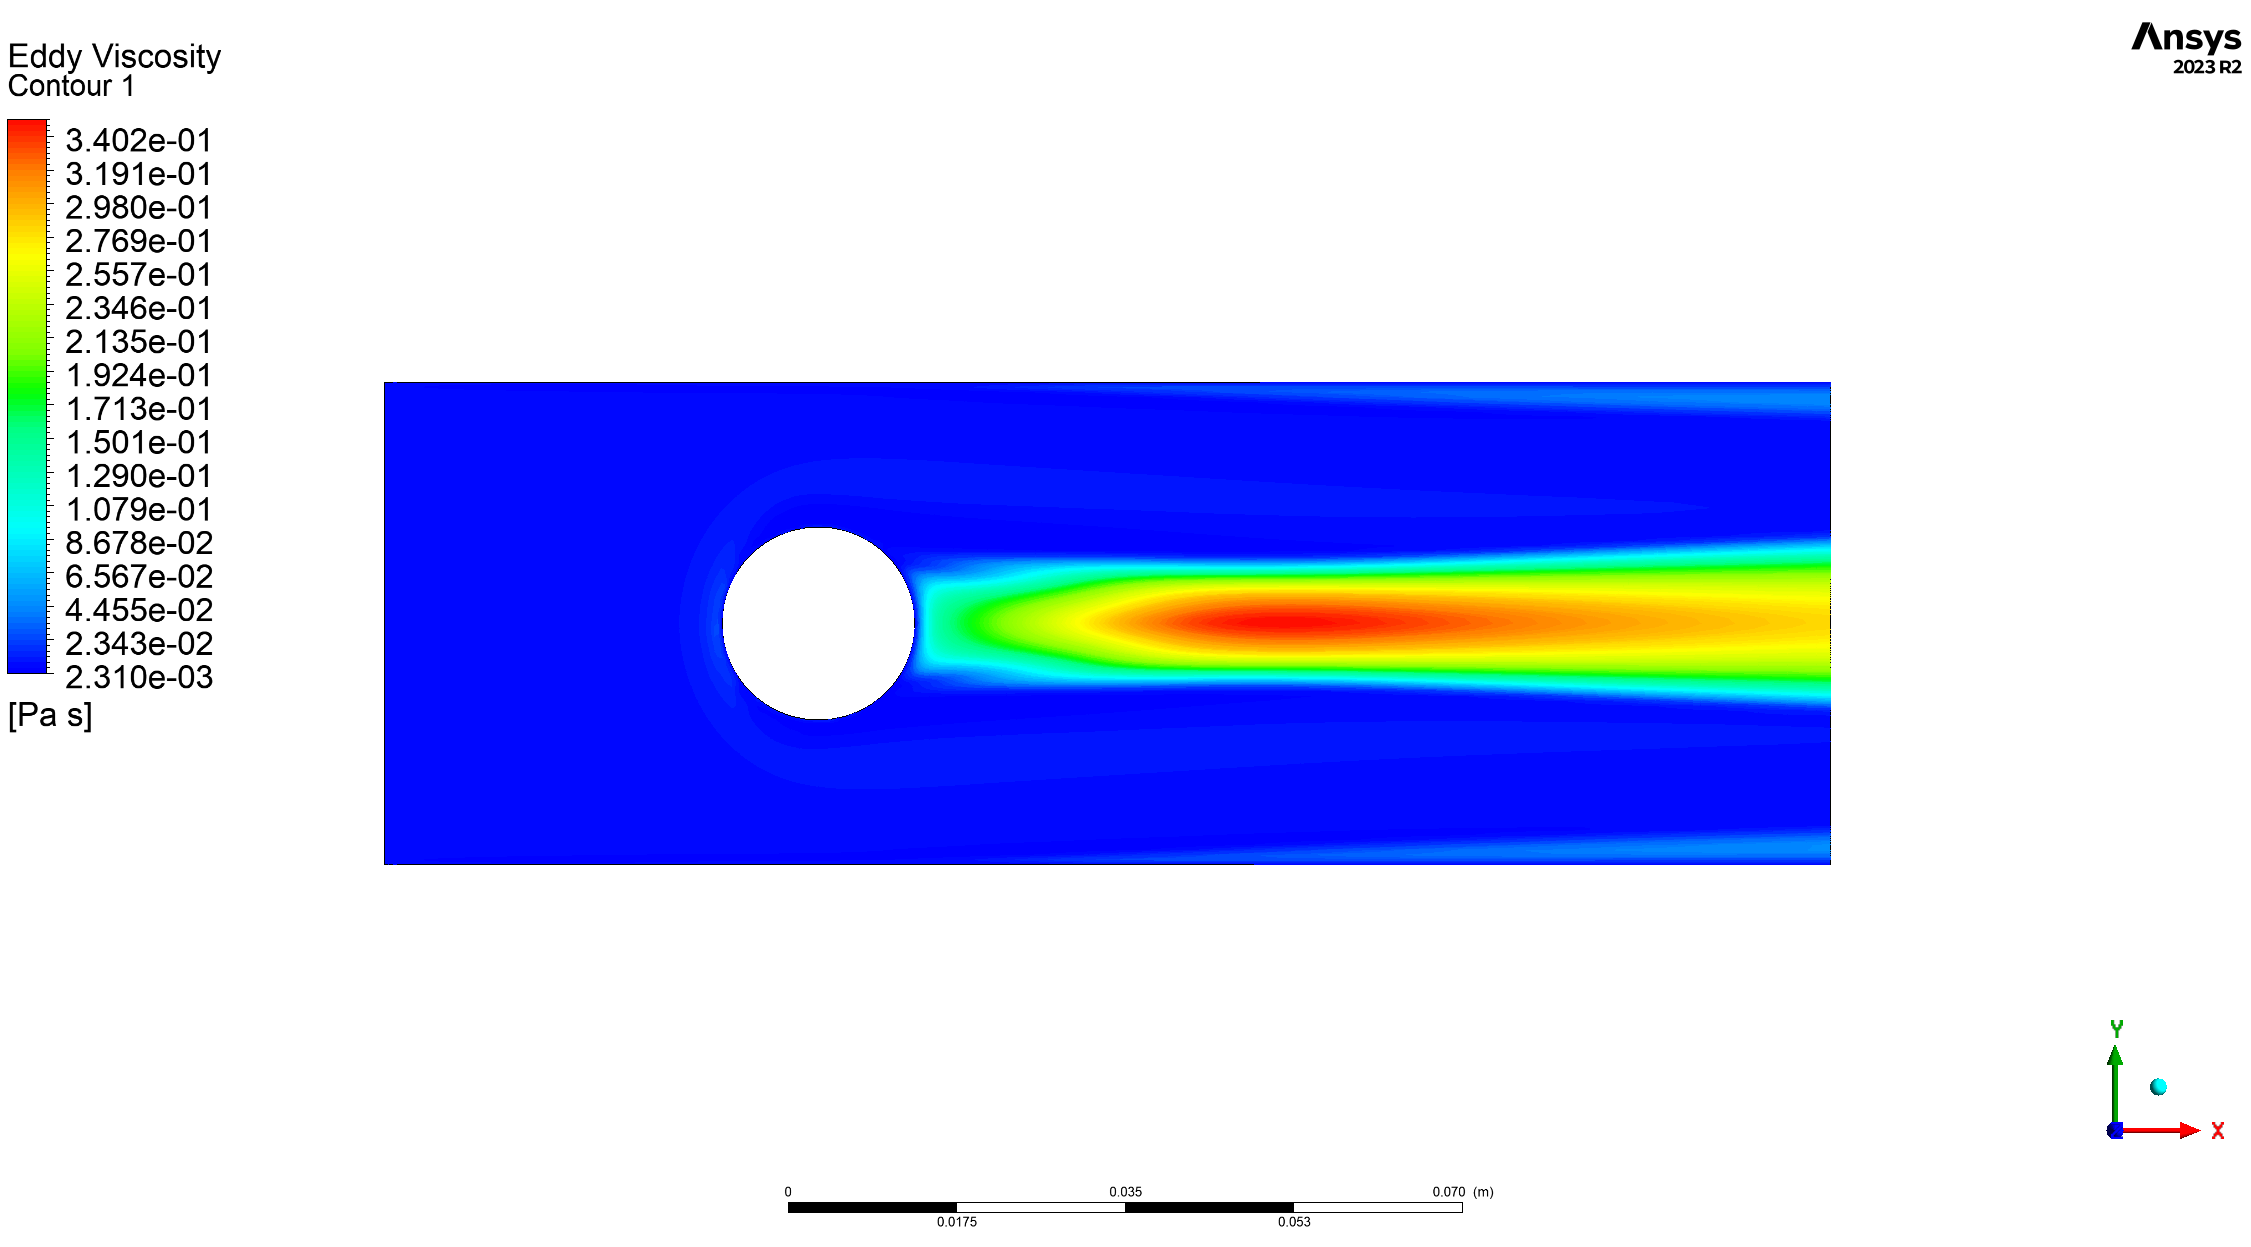
\includegraphics[width=0.45\textwidth]{papers/reynolds/images/eddy-viscosity.png}
  \caption{Eddy Viscosity ($\epsilon$-Feld)}
  \label{fig:e}
  \centering
  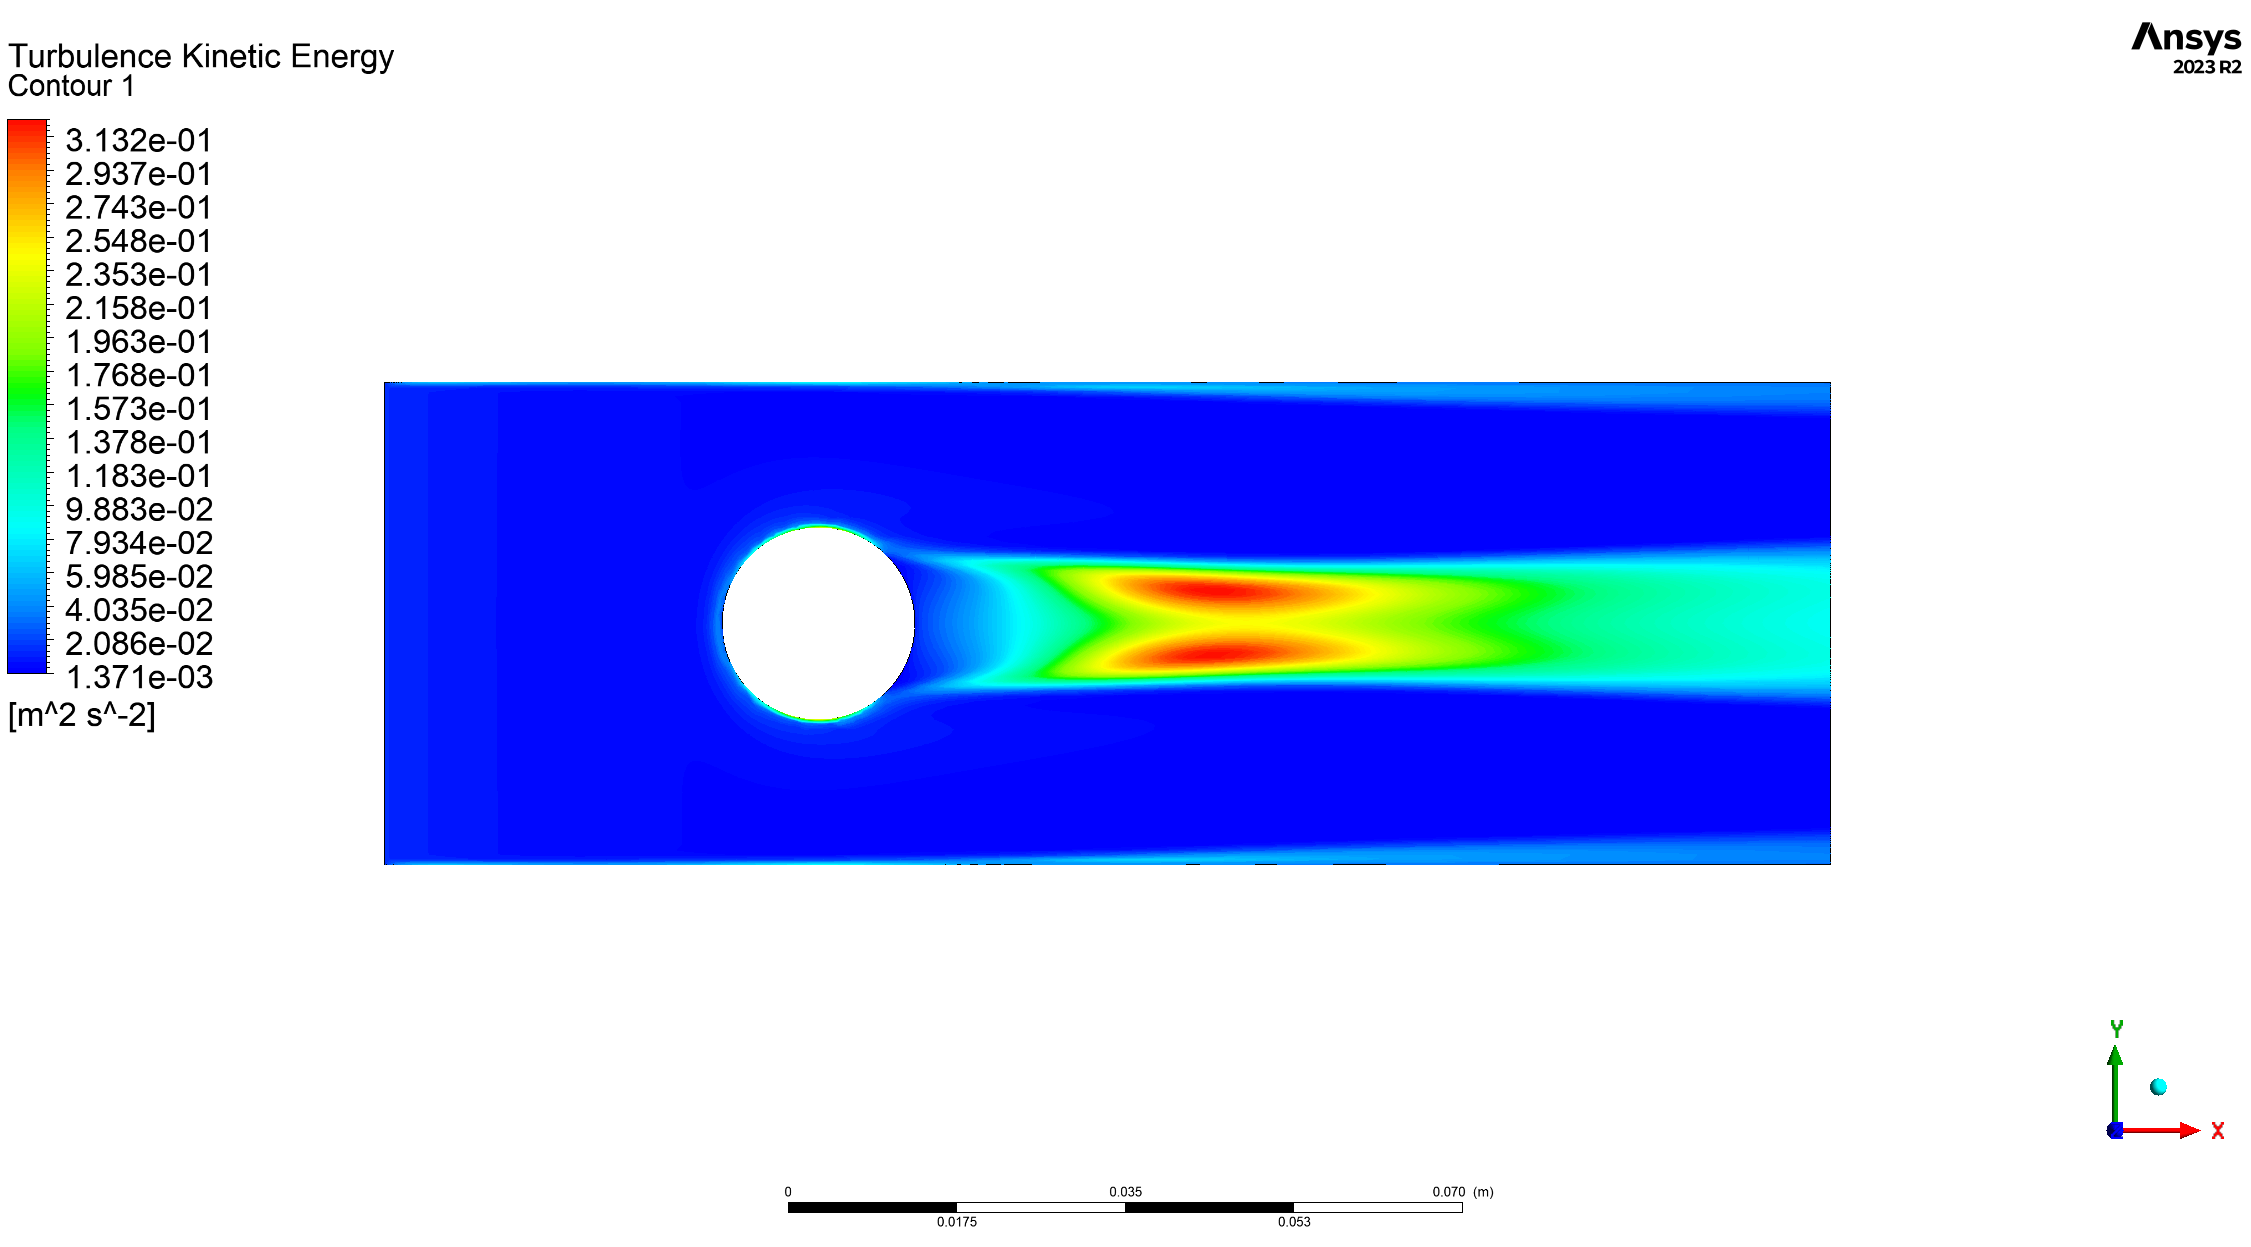
\includegraphics[width=0.45\textwidth]{papers/reynolds/images/turbulence-kinetic-energy.png}
  \caption{Turbulente Kinetische Ernergie (k-Feld)}
  \label{fig:k}
  \centering
  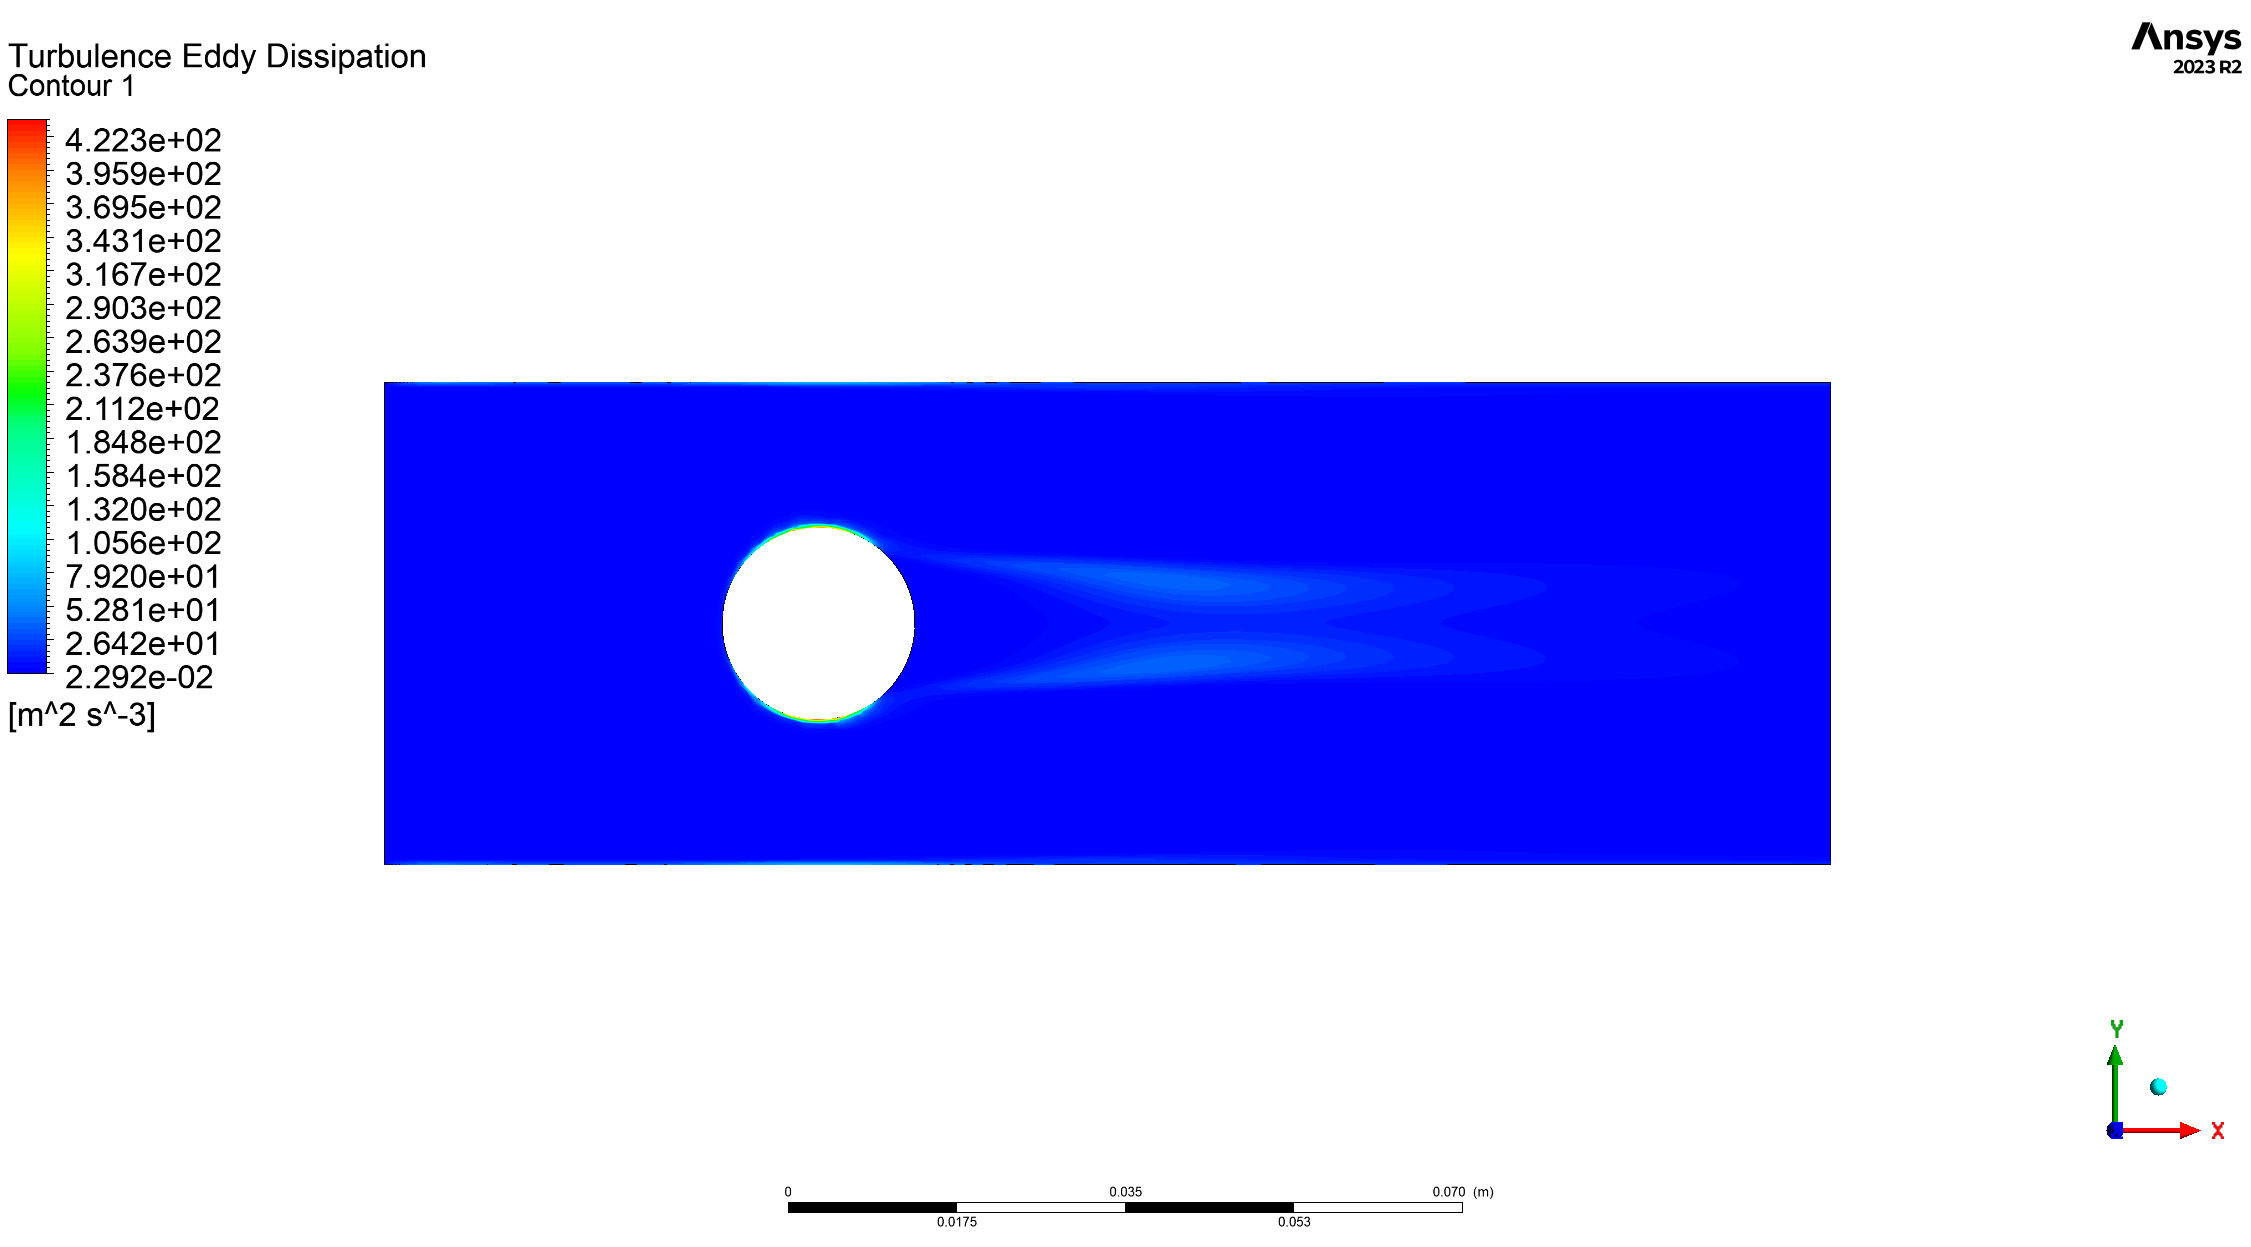
\includegraphics[width=0.45\textwidth]{papers/reynolds/images/turbulent-viscosity.png}
  \caption{Turbulente Viskosität}
  \label{fig:mu-t}
\end{figure}